\chapter{text}
\begin{figure}[H]
\centering
\begin{minipage}[t]{0.48\textwidth}
    \centering
    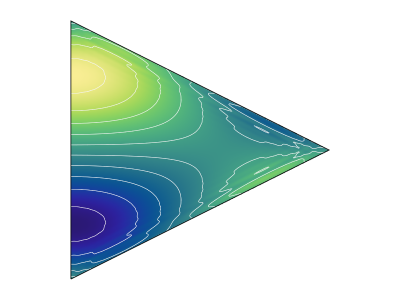
\includegraphics[width=6cm]{figure/Mxy/Gauss-Penalty.png}
\caption*{Gauss-Penalty}
\end{minipage}
\begin{minipage}[t]{0.48\textwidth}
    \centering
    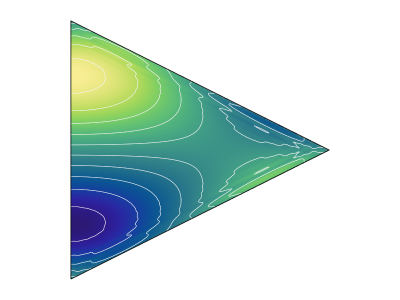
\includegraphics[width=6cm]{figure/Mxy/Gauss-Nitsche.png}
    \caption*{Gauss-Nitsche}
\end{minipage}
\begin{minipage}[t]{0.48\textwidth}
    \centering
        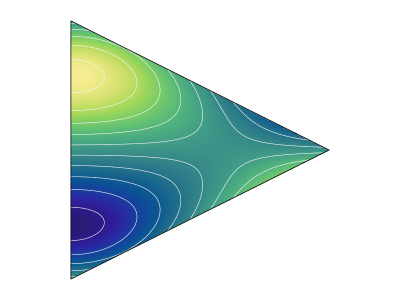
\includegraphics[width=6cm]{figure/Mxy/RKGSI-Penalty.png}
    \caption*{RKGSI-Penalty}
\end{minipage}
\begin{minipage}[t]{0.48\textwidth}
    \centering
        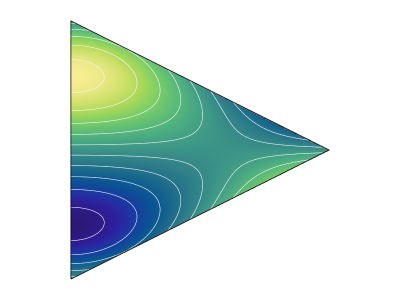
\includegraphics[width=6cm]{figure/Mxy/RKGSI-Nitsche.png}
        \caption*{RKGSI-Nitsche}
\end{minipage}
\begin{minipage}[t]{0.48\textwidth}
    \centering
        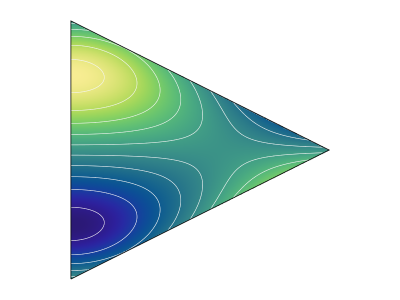
\includegraphics[width=6cm]{figure/Mxy/RKGSI-HR.png}
        \caption*{RKGSI-HR}
\end{minipage}
\begin{minipage}[t]{0.48\textwidth}
    \centering
        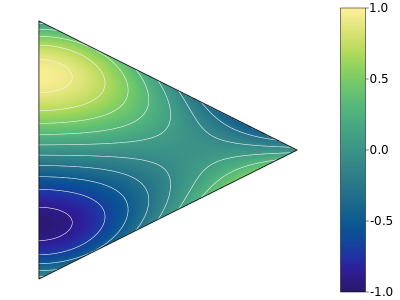
\includegraphics[width=5cm]{figure/Mxy/Exact-Solution.png}
        \caption*{Exact-Solution}
\end{minipage}
\caption{悬臂梁问题误差对比}
\label{ECLH}
\end{figure}
\begin{figure}[H]
    \centering
        \includegraphics[scale=0.1]{figure/PHR/T/Mxy1.png}
    \caption{简支等边三角形板问题弯矩云图$\sigma_{xx}$应力云图}
    \label{TMxy}
    \end{figure} 

